% Chapter 11: Economic Model
\chapter{Economic Model}
\label{ch:economics}

This chapter provides a comprehensive analysis of the economic properties, cost structures, and sustainability model of \tprotocol{}.

\section{Cost Structure Overview}
\label{sec:cost-overview}

\tprotocol{} introduces a fundamentally different cost model compared to traditional payment systems. The total cost of a payment consists of three components:

\begin{figure}[ht]
\centering
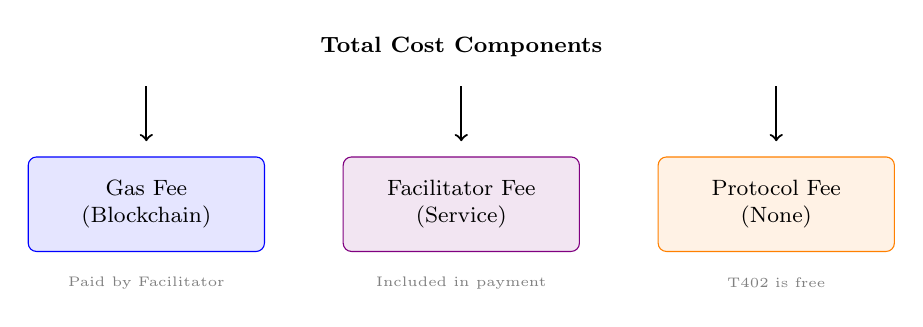
\begin{tikzpicture}[
    component/.style={
        rectangle,
        rounded corners=3pt,
        minimum width=3cm,
        minimum height=1.2cm,
        draw=blue,
        fill=blue!10,
        font=\footnotesize,
        align=center
    }
]

\node[component] (gas) at (0,0) {Gas Fee\\(Blockchain)};
\node[component, draw=violet, fill=violet!10] (facilitator) at (4,0) {Facilitator Fee\\(Service)};
\node[component, draw=orange, fill=orange!10] (protocol) at (8,0) {Protocol Fee\\(None)};

\node[font=\tiny, gray] at (0,-1) {Paid by Facilitator};
\node[font=\tiny, gray] at (4,-1) {Included in payment};
\node[font=\tiny, gray] at (8,-1) {T402 is free};

\draw[->, thick] (0,1.5) -- (0,0.8);
\draw[->, thick] (4,1.5) -- (4,0.8);
\draw[->, thick] (8,1.5) -- (8,0.8);

\node[font=\footnotesize\bfseries] at (4,2) {Total Cost Components};

\end{tikzpicture}
\caption{T402 cost structure}
\label{fig:cost-structure}
\end{figure}

\begin{table}[ht]
\centering
\caption{Cost Component Breakdown}
\label{tab:cost-breakdown}
\begin{tabular}{l l p{5.5cm}}
\toprule
\textbf{Component} & \textbf{Typical Cost} & \textbf{Who Pays} \\
\midrule
Gas Fee & \$0.001--0.10 & Facilitator (sponsored) \\
Facilitator Fee & 0--1\% & Deducted from payment \\
Protocol Fee & \$0.00 & N/A (open source) \\
\bottomrule
\end{tabular}
\end{table}

\section{Traditional Payment Comparison}
\label{sec:traditional-comparison}

\subsection{Fee Structure Comparison}

\begin{table}[ht]
\centering
\caption{Payment Provider Fee Comparison}
\label{tab:provider-comparison}
\footnotesize
\begin{tabular}{l r r r r}
\toprule
\textbf{Provider} & \textbf{Fixed Fee} & \textbf{\% Fee} & \textbf{Intl Fee} & \textbf{Settlement} \\
\midrule
Stripe & \$0.30 & 2.9\% & +1.5\% & 2 days \\
PayPal & \$0.49 & 3.49\% & +1.5\% & 1-3 days \\
Square & \$0.30 & 2.6\% & +1\% & 1-2 days \\
Adyen & \$0.12 & 2.9\% & +1\% & 3 days \\
T402 & \$0.00 & 0-1\% & 0\% & Instant \\
\bottomrule
\end{tabular}
\end{table}

\subsection{Cost by Transaction Size}

\begin{figure}[ht]
\centering
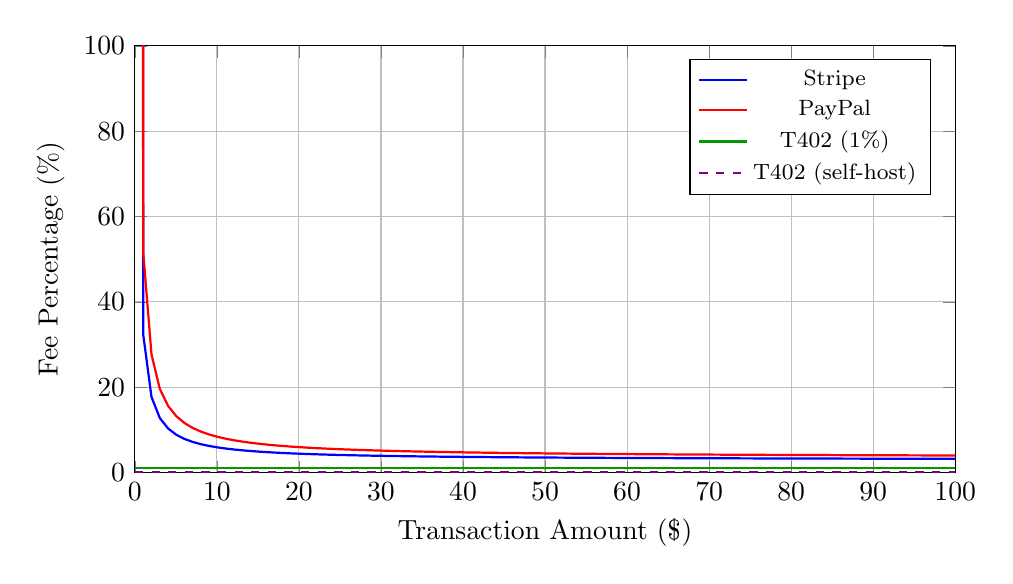
\begin{tikzpicture}
\begin{axis}[
    width=12cm,
    height=7cm,
    xlabel={Transaction Amount (\$)},
    ylabel={Fee Percentage (\%)},
    xmin=0, xmax=100,
    ymin=0, ymax=100,
    legend pos=north east,
    grid=major,
    legend style={font=\footnotesize}
]

% Stripe: 2.9% + $0.30
\addplot[color=blue, thick, domain=0.01:100, samples=100]
    {(0.30 + 0.029*x) / x * 100};
\addlegendentry{Stripe}

% PayPal: 3.49% + $0.49
\addplot[color=red, thick, domain=0.01:100, samples=100]
    {(0.49 + 0.0349*x) / x * 100};
\addlegendentry{PayPal}

% T402: 1% (flat)
\addplot[color=green!60!black, thick, domain=0.01:100]
    {1};
\addlegendentry{T402 (1\%)}

% T402: 0% (self-host)
\addplot[color=violet, thick, dashed, domain=0.01:100]
    {0.1};
\addlegendentry{T402 (self-host)}

\end{axis}
\end{tikzpicture}
\caption{Fee percentage by transaction size}
\label{fig:fee-comparison}
\end{figure}

\subsection{Break-Even Analysis}

\begin{table}[ht]
\centering
\caption{Break-Even: T402 vs Stripe}
\label{tab:breakeven}
\begin{tabular}{r r r r}
\toprule
\textbf{Amount} & \textbf{Stripe Fee} & \textbf{T402 Fee} & \textbf{Savings} \\
\midrule
\$0.01 & \$0.30 (3000\%) & \$0.0001 (1\%) & 99.97\% \\
\$0.10 & \$0.30 (303\%) & \$0.001 (1\%) & 99.67\% \\
\$1.00 & \$0.33 (33\%) & \$0.01 (1\%) & 96.97\% \\
\$5.00 & \$0.45 (8.9\%) & \$0.05 (1\%) & 88.89\% \\
\$10.00 & \$0.59 (5.9\%) & \$0.10 (1\%) & 83.05\% \\
\$50.00 & \$1.75 (3.5\%) & \$0.50 (1\%) & 71.43\% \\
\$100.00 & \$3.20 (3.2\%) & \$1.00 (1\%) & 68.75\% \\
\bottomrule
\end{tabular}
\end{table}

\begin{infobox}[Micropayment Sweet Spot]
\tprotocol{} provides the greatest advantage for payments under \$10, where traditional fixed fees dominate. For a \$0.10 payment, T402 is 300x more cost-effective than Stripe.
\end{infobox}

\section{Network Economics}
\label{sec:network-economics}

Different blockchain networks offer varying cost profiles:

\subsection{Gas Fee Comparison}

\begin{table}[ht]
\centering
\caption{Network Gas Fee Comparison (EIP-3009 Transfer)}
\label{tab:gas-comparison}
\footnotesize
\begin{tabular}{l r r r}
\toprule
\textbf{Network} & \textbf{Gas Units} & \textbf{Gas Price} & \textbf{USD Cost} \\
\midrule
Ethereum L1 & 65,000 & 30 gwei & \$4.50--15.00 \\
Arbitrum One & 65,000 & 0.1 gwei & \$0.01--0.05 \\
Base & 65,000 & 0.001 gwei & \$0.001--0.01 \\
Optimism & 65,000 & 0.001 gwei & \$0.001--0.01 \\
Solana & 5,000 CU & -- & \$0.0001 \\
TON & -- & -- & \$0.01--0.05 \\
TRON & 30,000 & -- & \$0.10--0.50 \\
\bottomrule
\end{tabular}
\end{table}

\subsection{Network Selection Matrix}

\begin{figure}[ht]
\centering
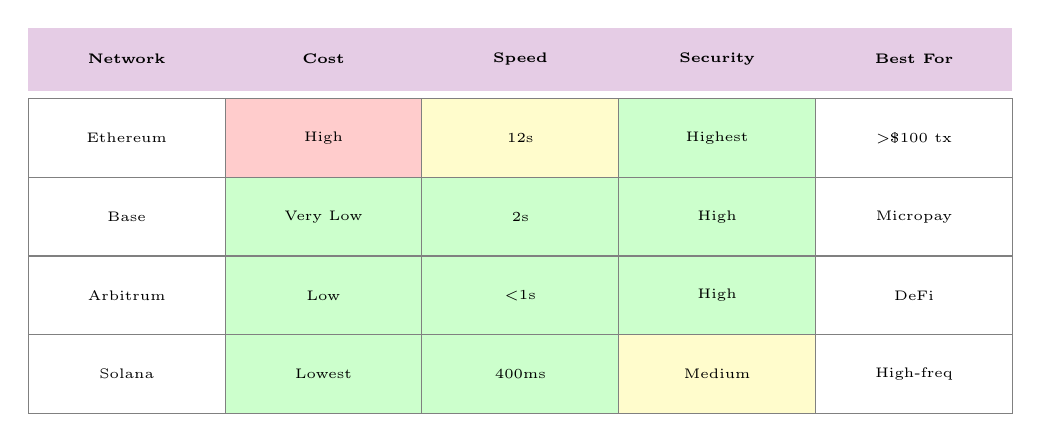
\begin{tikzpicture}[
    cell/.style={
        rectangle,
        minimum width=2.5cm,
        minimum height=1cm,
        draw=gray,
        font=\tiny,
        align=center
    },
    header/.style={
        rectangle,
        minimum width=2.5cm,
        minimum height=0.8cm,
        fill=violet!20,
        font=\tiny\bfseries,
        align=center
    },
    good/.style={fill=green!20},
    medium/.style={fill=yellow!20},
    poor/.style={fill=red!20}
]

% Headers
\node[header] at (0,2.5) {Network};
\node[header] at (2.5,2.5) {Cost};
\node[header] at (5,2.5) {Speed};
\node[header] at (7.5,2.5) {Security};
\node[header] at (10,2.5) {Best For};

% Ethereum
\node[cell] at (0,1.5) {Ethereum};
\node[cell, poor] at (2.5,1.5) {High};
\node[cell, medium] at (5,1.5) {12s};
\node[cell, good] at (7.5,1.5) {Highest};
\node[cell] at (10,1.5) {>\$100 tx};

% Base
\node[cell] at (0,0.5) {Base};
\node[cell, good] at (2.5,0.5) {Very Low};
\node[cell, good] at (5,0.5) {2s};
\node[cell, good] at (7.5,0.5) {High};
\node[cell] at (10,0.5) {Micropay};

% Arbitrum
\node[cell] at (0,-0.5) {Arbitrum};
\node[cell, good] at (2.5,-0.5) {Low};
\node[cell, good] at (5,-0.5) {<1s};
\node[cell, good] at (7.5,-0.5) {High};
\node[cell] at (10,-0.5) {DeFi};

% Solana
\node[cell] at (0,-1.5) {Solana};
\node[cell, good] at (2.5,-1.5) {Lowest};
\node[cell, good] at (5,-1.5) {400ms};
\node[cell, medium] at (7.5,-1.5) {Medium};
\node[cell] at (10,-1.5) {High-freq};

\end{tikzpicture}
\caption{Network selection matrix}
\label{fig:network-matrix}
\end{figure}

\section{Facilitator Economics}
\label{sec:facilitator-economics}

The Facilitator service operates as the economic bridge between users and blockchain networks.

\subsection{Revenue Model}

\begin{table}[ht]
\centering
\caption{Facilitator Revenue Sources}
\label{tab:facilitator-revenue}
\begin{tabular}{l l p{5cm}}
\toprule
\textbf{Source} & \textbf{Rate} & \textbf{Description} \\
\midrule
Settlement Fee & 0--1\% & Per-transaction fee \\
Priority Processing & Fixed & Guaranteed fast settlement \\
Enterprise SLA & Monthly & Dedicated infrastructure \\
White-label & License & Self-hosted deployment \\
\bottomrule
\end{tabular}
\end{table}

\subsection{Cost Structure}

\begin{table}[ht]
\centering
\caption{Facilitator Operating Costs}
\label{tab:facilitator-costs}
\begin{tabular}{l r p{4.5cm}}
\toprule
\textbf{Category} & \textbf{Monthly} & \textbf{Notes} \\
\midrule
Infrastructure & \$500--2,000 & Servers, databases \\
RPC Services & \$200--1,000 & Alchemy, QuickNode \\
Gas Reserves & Variable & Based on volume \\
Monitoring & \$100--500 & Grafana, alerts \\
Security & \$200--1,000 & Audits, HSM \\
\bottomrule
\end{tabular}
\end{table}

\subsection{Break-Even Volume}

\begin{figure}[ht]
\centering
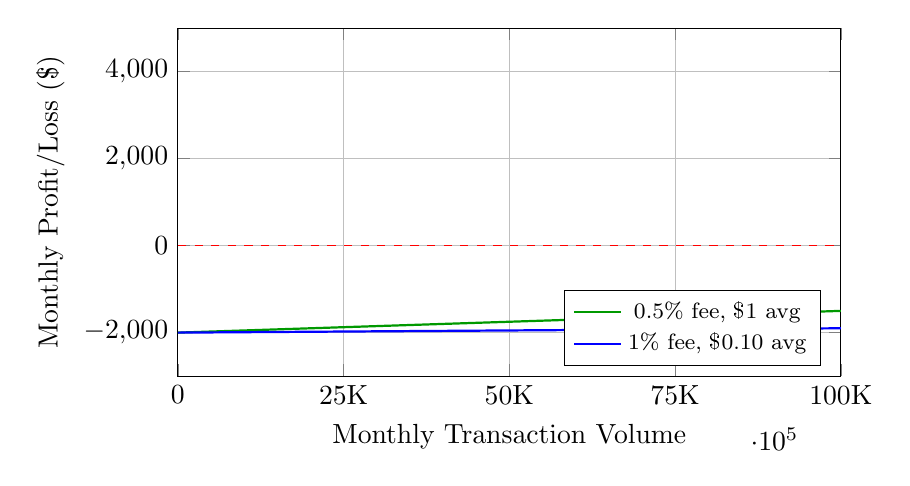
\begin{tikzpicture}
\begin{axis}[
    width=10cm,
    height=6cm,
    xlabel={Monthly Transaction Volume},
    ylabel={Monthly Profit/Loss (\$)},
    xmin=0, xmax=100000,
    ymin=-3000, ymax=5000,
    legend pos=south east,
    grid=major,
    legend style={font=\footnotesize},
    xtick={0,25000,50000,75000,100000},
    xticklabels={0,25K,50K,75K,100K}
]

% Revenue (0.5% of $1 avg transaction)
\addplot[color=green!60!black, thick, domain=0:100000]
    {x * 0.005 - 2000};
\addlegendentry{0.5\% fee, \$1 avg}

% Revenue (1% of $0.10 avg transaction)
\addplot[color=blue, thick, domain=0:100000]
    {x * 0.001 - 2000};
\addlegendentry{1\% fee, \$0.10 avg}

% Break-even line
\addplot[color=red, dashed, domain=0:100000] {0};

\end{axis}
\end{tikzpicture}
\caption{Facilitator break-even analysis}
\label{fig:facilitator-breakeven}
\end{figure}

\section{Token Economics}
\label{sec:token-economics}

\subsection{USDT vs USDC Comparison}

\begin{table}[ht]
\centering
\caption{Stablecoin Comparison}
\label{tab:stablecoin-comparison}
\footnotesize
\begin{tabular}{l r r r}
\toprule
\textbf{Property} & \textbf{USDT} & \textbf{USDC} & \textbf{USDT0} \\
\midrule
Market Cap & \$120B+ & \$30B+ & -- \\
Daily Volume & \$50B+ & \$5B+ & -- \\
Chains Supported & 15+ & 10+ & 20+ (OFT) \\
EIP-3009 Support & Yes & Yes & Yes \\
Cross-chain Native & No & No & Yes \\
\bottomrule
\end{tabular}
\end{table}

\subsection{USDT0 LayerZero Economics}

USDT0 provides native cross-chain transfers via LayerZero:

\begin{itemize}
    \item \textbf{No Bridge Fees}: Native OFT transfer vs bridge fees
    \item \textbf{Unified Liquidity}: Same token across all chains
    \item \textbf{Fast Settlement}: Minutes vs hours for bridges
    \item \textbf{Lower Risk}: No bridge exploits possible
\end{itemize}

\section{Volume Economics}
\label{sec:volume-economics}

\subsection{Economies of Scale}

\begin{table}[ht]
\centering
\caption{Cost Optimization by Volume}
\label{tab:volume-optimization}
\footnotesize
\begin{tabular}{r r r r}
\toprule
\textbf{Monthly Volume} & \textbf{Avg Gas/Tx} & \textbf{Effective Rate} & \textbf{Savings vs Stripe} \\
\midrule
1,000 tx & \$0.01 & 2.0\% & 50\% \\
10,000 tx & \$0.005 & 1.5\% & 60\% \\
100,000 tx & \$0.002 & 1.2\% & 65\% \\
1,000,000 tx & \$0.001 & 1.0\% & 70\% \\
\bottomrule
\end{tabular}
\end{table}

\subsection{Batch Settlement Optimization}

High-volume operators can reduce costs through batching:

\begin{lstlisting}[language=typescript,caption={Batch settlement for cost optimization}]
// Configure batch settlement
const config = {
  batchSize: 100,           // Settle 100 tx per batch
  maxWaitTime: 60000,       // Max 60 seconds
  minBatchValue: "100000",  // Min $0.10 per batch
};

// Cost savings:
// - Single tx: $0.01 gas
// - Batch of 100: $0.02 gas total
// - Savings: 98% on gas costs
\end{lstlisting}

\section{ROI Analysis}
\label{sec:roi-analysis}

\subsection{API Provider Example}

\begin{table}[ht]
\centering
\caption{ROI: Weather API Provider}
\label{tab:roi-weather}
\begin{tabular}{l r r}
\toprule
\textbf{Metric} & \textbf{Stripe} & \textbf{T402} \\
\midrule
Monthly API Calls & 1,000,000 & 1,000,000 \\
Price per Call & \$0.001 & \$0.001 \\
Gross Revenue & \$1,000 & \$1,000 \\
Payment Fees & \$300+ & \$10 \\
Net Revenue & \$700 & \$990 \\
\textbf{Effective Margin} & \textbf{70\%} & \textbf{99\%} \\
\bottomrule
\end{tabular}
\end{table}

\begin{warningbox}[Traditional Limitation]
With Stripe's \$0.30 minimum fee, the weather API would need to charge at least \$0.50 per call to be viable---500x higher than market rates.
\end{warningbox}

\subsection{Content Platform Example}

\begin{table}[ht]
\centering
\caption{ROI: News Platform Pay-Per-Article}
\label{tab:roi-news}
\begin{tabular}{l r r}
\toprule
\textbf{Metric} & \textbf{Subscription} & \textbf{T402 PPV} \\
\midrule
Monthly Users & 10,000 & 50,000 \\
Conversion Rate & 2\% & 15\% \\
Paying Users & 200 & 7,500 \\
Avg Revenue/User & \$10.00 & \$0.75 \\
Gross Revenue & \$2,000 & \$5,625 \\
Payment Fees & \$118 & \$56 \\
\textbf{Net Revenue} & \textbf{\$1,882} & \textbf{\$5,569} \\
\bottomrule
\end{tabular}
\end{table}

\section{Market Opportunity}
\label{sec:market-opportunity}

\subsection{Total Addressable Market}

\begin{figure}[ht]
\centering
\begin{tikzpicture}[
    circle/.style={
        ellipse,
        draw=violet,
        thick,
        font=\footnotesize,
        align=center
    }
]

\node[circle, minimum width=8cm, minimum height=4cm, fill=violet!5] (tam) at (0,0) {};
\node[circle, minimum width=5.5cm, minimum height=2.8cm, fill=violet!15] (sam) at (0,-0.3) {};
\node[circle, minimum width=3cm, minimum height=1.5cm, fill=violet!30] (som) at (0,-0.5) {};

\node[font=\footnotesize] at (0,1.5) {TAM: \$500B+};
\node[font=\tiny, gray] at (0,1.1) {Global digital payments};

\node[font=\footnotesize] at (0,0.3) {SAM: \$50B};
\node[font=\tiny, gray] at (0,-0.1) {API/Micropayments};

\node[font=\footnotesize] at (0,-0.7) {SOM: \$1B};
\node[font=\tiny, gray] at (0,-1.1) {Crypto-native};

\end{tikzpicture}
\caption{Market opportunity sizing}
\label{fig:market-sizing}
\end{figure}

\subsection{Growth Segments}

\begin{table}[ht]
\centering
\caption{High-Growth Market Segments}
\label{tab:growth-segments}
\begin{tabular}{l r r}
\toprule
\textbf{Segment} & \textbf{2024 Size} & \textbf{CAGR} \\
\midrule
AI Agent Services & \$2B & 85\% \\
API Economy & \$15B & 25\% \\
Creator Economy & \$100B & 20\% \\
IoT Payments & \$5B & 40\% \\
Cross-border Freelance & \$50B & 15\% \\
\bottomrule
\end{tabular}
\end{table}

\section{Economic Sustainability}
\label{sec:sustainability}

\subsection{Long-term Viability}

\tprotocol{}'s economic sustainability is ensured by:

\begin{enumerate}
    \item \textbf{Open Protocol}: No protocol fees, community-driven
    \item \textbf{Facilitator Competition}: Multiple providers ensure competitive fees
    \item \textbf{Chain Agnosticism}: Not dependent on single network
    \item \textbf{Stablecoin Diversity}: Support for multiple stablecoins
\end{enumerate}

\subsection{Risk Mitigation}

\begin{table}[ht]
\centering
\caption{Economic Risk Factors}
\label{tab:economic-risks}
\begin{tabular}{l p{4.5cm} p{4cm}}
\toprule
\textbf{Risk} & \textbf{Impact} & \textbf{Mitigation} \\
\midrule
L2 Fee Spikes & Increased settlement cost & Multi-chain support \\
Stablecoin Depeg & Payment value mismatch & Multi-stablecoin support \\
Facilitator Failure & Service disruption & Self-hosting option \\
Regulatory Change & Operational restrictions & Geographic diversity \\
\bottomrule
\end{tabular}
\end{table}

